\documentclass[12pt]{amsart}
\usepackage[utf8]{inputenc}
\usepackage[
backend=biber,
style=numeric,
maxbibnames=99,
sorting=ynt
]{biblatex}
\usepackage{amsmath,amssymb,amsthm}
\usepackage{tikz}
\usepackage{standalone}
\usepackage{svg}
\usepackage{gensymb}
\usepackage{float}
\usepackage{geometry}
\usepackage{hyperref}
\usepackage{graphicx, animate}
\usepackage{caption, subcaption}
\usepackage{pgffor}
\usepackage{mathtools}
\usepackage{array}
\addbibresource{bibliography.bib}
\usepackage{hyperref,thmtools}
\linespread{1.5}

% Override ugly default link
\hypersetup{
  colorlinks   = true, %Colours links instead of ugly boxes
  urlcolor     = blue, %Colour for external hyperlinks
  linkcolor    = blue, %Colour of internal links
  citecolor   = blue    %Colour of citations
}

\begin{document}

% \begin{section}{Introduction}
%     The modelling of temporal networks is an important task in many real world applications including symptom interactions for mental health \cite{jordan2020current,contreras2020temporal}, epidemiology \cite{masuda2013predicting}, and protein interactions \cite{lucas2021inferring,jin2009identifying}.
%     Temporal networks can be seen as dynamical systems: that is a system in which we have points, in our case nodes in a network, whose states, the edges connecting them, that vary dependent in time.
%     Discovering the underlying equations governing these dynamical systems proves challenging, because changes in network structure are typically observed in the form of discrete jumps from one state to another, for example an edge between two nodes not being observed at the first time step then appearing at the next.
%     Here, we propose a hybrid statistical and deep learning framework that allows us to model temporal networks as continuous-time dynamical systems, discover a fitting set of differential equations describing it, and, exploiting that discovery, predict the time evolution of a network.

%     Differential equations are useful for modelling systems where the state of one variable can effect the trajectories of other variables. We observe this behavior in temporal networks; nodes' connections within the network can influence the formation and decay of edges between other nodes, for example the phenomenon of preferential attachment observed in \cite{newman2001clustering,capocci2006preferential}, where a node is more lively to gain the connections the more connections it has. With this in mind we might wish to draw on the rich mathematical literature of differential equation modelling.

%     In the common representation of networks as binary-valued adjacency matrices, the events recorded in a temporal sequence of networks correspond to topological events, such as the appearance or the disappearance of link.
%     Because of the discrete nature of events, directly modelling the temporal networks as dynamical systems would require us to handle discrete jumps.
%     The topological nature of temporal networks, and the discontinuous character of their temporal evolution, make it challenging to use differential equations techniques.

%     Here, we overcome the discreteness problem by interpreting networks as Random Dot Product Graphs; a well established statistical model for complex networks, that embeds nodes in a continuous, low-dimensional metric space by using a truncated singular value decomposition\cite{athreya2017statistical}. In this way we translate the hard problem of modelling discrete events in the space of networks to the easier problem of modelling continuous change in the embedding space. We then define and use systems of Neural Network Differential Equations (NNDE)\cite{SciML_C_Rak} to approximate the time evolution of the embedding space, and symbolic regression techniques to discover the functional form of the fitted NNDEs. These functional forms are interpretable (as they read as classic differential equations) and allow us to predict forward in time the evolution of the temporal networks.

%     In this manuscript, we prove that the temporal network prediction problem can be successfully re-interpreted as a dynamical system modelling problem by taking the singular value decomposition of a sequence of adjacency matrices and training a NNDE to model an approximation to the underlying differential equation. We then go on to create a symbolic equation of this approximation. 

%     We apply our proposed framework to three small example temporal networks with the hope of exploring the limitations and strengths of the proposed framework. 
%     The framework we are introducing is extremely flexible, and our research regarding the optimal structure of the Neural Networks used for the NNDEs is just started.
%     We are confident that future research can identify more fitting Neural Network structures than the simple one adopted here.
%     For this reason, we did not yet attempt to benchmark our model against other classic temporal network prediction methods.
%     As it is completely general, we believe that the framework we are introducing can be usefully applied to areas of medicine, especially protein interaction networks; population dynamics for network ecology; and social network modelling. In particular, we discuss how specific domain knowledge relative to the prediction scenario can be taken into account, moving from NNDEs to Universal Differential Equations.
% \end{section}

% \begin{section}{Methodology}

%         We are given a sequence of graphs, and our goal is to predict the next graph in the sequence. To achieve this, we reinterpret each graph as a sequence of points in a latent space; that is, a space in which similar vertices (ones with many of the same neighbours) are mapped to a similar point in space. We then Train a Neural Network Differential Equation (NNDE) to approximate the rate of change of the points in this latent space. With this numerical equation we can then use symbolic regression techniques to find a functional equation that matches the numerical equation. Using this process we discover an interpretable function that governs the evolution of a differential equation.

%         \begin{figure}
%             \centering
%             \begin{subfigure}[c]{1\textwidth}
%                 \begin{tabular}{llll}
%                 \begin{subfigure}[c]{0.25\textwidth}
%                     \centering
%                     \resizebox{.6\width}{!}{\documentclass{standalone}
\usepackage{amsmath,amssymb,amsthm}
\usepackage{tikz}
\usetikzlibrary{decorations.markings}
\usetikzlibrary{arrows,automata}
\usetikzlibrary{positioning}
\usetikzlibrary{arrows.meta,positioning}

\begin{document}
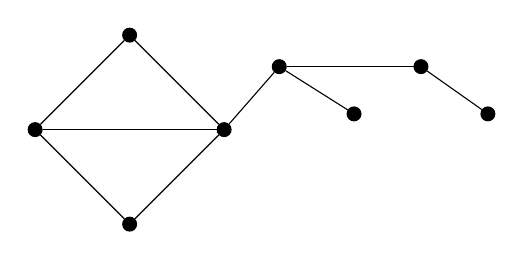
\begin{tikzpicture}[
    mycircle/.style={
        circle,
        draw=black,
        fill=black,
        fill opacity = 1,
        inner sep=0pt,
        minimum size=5pt,
        font=\small},
    nocircle/.style={
        circle,
        draw=black,
        fill=black,
        fill opacity = 1,
        inner sep=0pt,
        minimum size=0.45pt,
        font=\small},
    targetcircle/.style={
        circle,
        draw=red,
        fill=red,
        fill opacity = 1,
        inner sep=0pt,
        minimum size=5pt,
        font=\small},
    myarrow/.style={-},
    dottedarrow/.style={-,dashed},
    thiccarrow/.style={-,line width=0.9pt},
    node distance=1.2cm and 1.5cm
]

\begin{scope}
    \begin{scope}[rotate=90]
        \foreach \x/\y in {0/0,90/1,180/2, 270/3}{ % color in outer layer
        \node[mycircle] (\y) at (canvas polar cs: radius=1.2cm,angle=\x){};
        }
    \end{scope}

    \path[every node/.style={font=\sffamily\small}]
        % (0) edge [color=black] (1)
        (0) edge [color=black] (1)
        (0) edge [color=black] (3)
        (1) edge [color=black] (2)
        (1) edge [color=black] (3)
        (2) edge [color=black] (3);

    \node[mycircle] (a) at (1.9, 0.8) {};
    \node[mycircle] (b) at (2.85, 0.2) {};
    \node[mycircle] (c) at (3.7, 0.8) {};
    \node[mycircle] (d) at (4.55, 0.2) {};

    \path[every node/.style={font=\sffamily\small}]
        (3) edge [color=black] (a)
        (a) edge [color=black] (b)
        (a) edge [color=black] (c)
        (c) edge [color=black] (d);


\end{scope}
\end{tikzpicture}
\end{document}}
%                     \label{method net, a}
%                 \end{subfigure}
%                 &
%                 \centering
%                 \begin{subfigure}[c]{0.25\textwidth}
%                     \centering
%                     \resizebox{.6\width}{!}{\documentclass{standalone}
\usepackage{amsmath,amssymb,amsthm}
\usepackage{tikz}
\usetikzlibrary{decorations.markings}
\usetikzlibrary{arrows,automata}
\usetikzlibrary{positioning}
\usetikzlibrary{arrows.meta,positioning}

\begin{document}
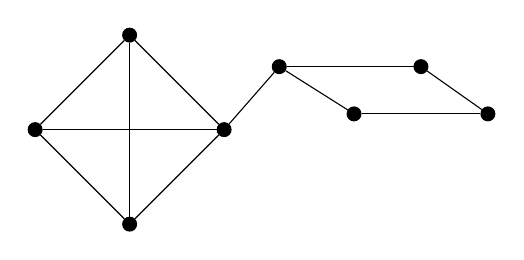
\begin{tikzpicture}[
    mycircle/.style={
        circle,
        draw=black,
        fill=black,
        fill opacity = 1,
        inner sep=0pt,
        minimum size=5pt,
        font=\small},
    nocircle/.style={
        circle,
        draw=black,
        fill=black,
        fill opacity = 1,
        inner sep=0pt,
        minimum size=0.45pt,
        font=\small},
    targetcircle/.style={
        circle,
        draw=red,
        fill=red,
        fill opacity = 1,
        inner sep=0pt,
        minimum size=5pt,
        font=\small},
    myarrow/.style={-},
    dottedarrow/.style={-,dashed},
    thiccarrow/.style={-,line width=0.9pt},
    node distance=1.2cm and 1.5cm
]

\begin{scope}
    \begin{scope}[rotate=90]
        \foreach \x/\y in {0/0,90/1,180/2, 270/3}{ % color in outer layer
        \node[mycircle] (\y) at (canvas polar cs: radius=1.2cm,angle=\x){};
        }
    \end{scope}

    \path[every node/.style={font=\sffamily\small}]
        % (0) edge [color=black] (1)
        (0) edge [color=black] (1)
        (0) edge [color=black] (2)
        (0) edge [color=black] (3)
        (1) edge [color=black] (2)
        (1) edge [color=black] (3)
        (2) edge [color=black] (3);

    \node[mycircle] (a) at (1.9, 0.8) {};
    \node[mycircle] (b) at (2.85, 0.2) {};
    \node[mycircle] (c) at (3.7, 0.8) {};
    \node[mycircle] (d) at (4.55, 0.2) {};

    \path[every node/.style={font=\sffamily\small}]
        (3) edge [color=black] (a)
        (a) edge [color=black] (b)
        (a) edge [color=black] (c)
        (c) edge [color=black] (d)
        (b) edge [color=black] (d);


\end{scope}
\end{tikzpicture}
\end{document}}
%                     \label{method net, b}
%                 \end{subfigure}
%                 &
%                 $\cdots$
%                 &
%                 \centering
%                 \begin{subfigure}[c]{0.25\textwidth}
%                     \centering
%                     \resizebox{.6\width}{!}{\documentclass{standalone}
\usepackage{amsmath,amssymb,amsthm}
\usepackage{tikz}
\usetikzlibrary{decorations.markings}
\usetikzlibrary{arrows,automata}
\usetikzlibrary{positioning}
\usetikzlibrary{arrows.meta,positioning}

\begin{document}
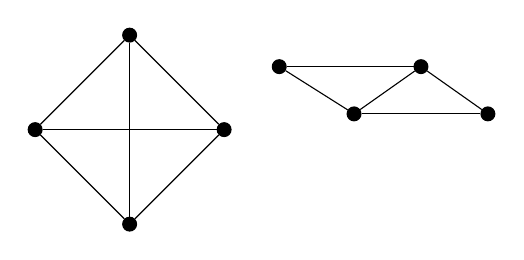
\begin{tikzpicture}[
    mycircle/.style={
        circle,
        draw=black,
        fill=black,
        fill opacity = 1,
        inner sep=0pt,
        minimum size=5pt,
        font=\small},
    nocircle/.style={
        circle,
        draw=black,
        fill=black,
        fill opacity = 1,
        inner sep=0pt,
        minimum size=0.45pt,
        font=\small},
    targetcircle/.style={
        circle,
        draw=red,
        fill=red,
        fill opacity = 1,
        inner sep=0pt,
        minimum size=5pt,
        font=\small},
    myarrow/.style={-},
    dottedarrow/.style={-,dashed},
    thiccarrow/.style={-,line width=0.9pt},
    node distance=1.2cm and 1.5cm
]

\begin{scope}
    \begin{scope}[rotate=90]
        \foreach \x/\y in {0/0,90/1,180/2, 270/3}{ % color in outer layer
        \node[mycircle] (\y) at (canvas polar cs: radius=1.2cm,angle=\x){};
        }
    \end{scope}

    \path[every node/.style={font=\sffamily\small}]
        % (0) edge [color=black] (1)
        (0) edge [color=black] (1)
        (0) edge [color=black] (2)
        (0) edge [color=black] (3)
        (1) edge [color=black] (2)
        (1) edge [color=black] (3)
        (2) edge [color=black] (3);

    \node[mycircle] (a) at (1.9, 0.8) {};
    \node[mycircle] (b) at (2.85, 0.2) {};
    \node[mycircle] (c) at (3.7, 0.8) {};
    \node[mycircle] (d) at (4.55, 0.2) {};

    \path[every node/.style={font=\sffamily\small}]
        (b) edge [color=black] (c)
        (a) edge [color=black] (b)
        (a) edge [color=black] (c)
        (c) edge [color=black] (d)
        (b) edge [color=black] (d);


\end{scope}
\end{tikzpicture}
\end{document}}
%                     \label{method net, c}
%                 \end{subfigure}
                
%                 \end{tabular}
%                 \caption{Example sequence of networks.}
%                 \label{method nets}
                
%             \end{subfigure}
%             \begin{subfigure}[c]{1\textwidth}
%                 \begin{tabular}{llll}
%                     $\begin{bmatrix}
%                         \cdot & 1 & 1 & 1 & \cdot & \cdot & \cdot & \cdot\\
%                         1 & \cdot & 1 & \cdot & \cdot & \cdot & \cdot & \cdot\\
%                         1 & 1 & \cdot & 1 & 1 & \cdot & \cdot & \cdot\\
%                         1 & \cdot & 1 & \cdot & \cdot & \cdot & \cdot & \cdot\\
%                         \cdot & \cdot & 1 & \cdot & \cdot & 1 & 1 & \cdot\\
%                         \cdot & \cdot & \cdot & \cdot & 1 & \cdot & \cdot & \cdot\\
%                         \cdot & \cdot & \cdot & \cdot & 1 & \cdot & \cdot & 1\\
%                         \cdot & \cdot & \cdot & \cdot & \cdot & \cdot & 1 & \cdot
%                     \end{bmatrix}$
%                     &
%                     $\begin{bmatrix}
%                         \cdot & 1 & 1 & 1 & \cdot & \cdot & \cdot & \cdot\\
%                         1 & \cdot & 1 & 1 & \cdot & \cdot & \cdot & \cdot\\
%                         1 & 1 & \cdot & 1 & 1 & \cdot & \cdot & \cdot\\
%                         1 & 1 & 1 & \cdot & \cdot & \cdot & \cdot & \cdot\\
%                         \cdot & \cdot & 1 & \cdot & \cdot & 1 & 1 & \cdot\\
%                         \cdot & \cdot & \cdot & \cdot & 1 & \cdot & \cdot & 1\\
%                         \cdot & \cdot & \cdot & \cdot & 1 & \cdot & \cdot & 1\\
%                         \cdot & \cdot & \cdot & \cdot & \cdot & 1 & 1 & \cdot
%                     \end{bmatrix}$
%                     &
%                     $\cdots$
%                     &
%                     $\begin{bmatrix}
%                         \cdot & 1 & 1 & 1 & \cdot & \cdot & \cdot & \cdot\\
%                         1 & \cdot & 1 & 1 & \cdot & \cdot & \cdot & \cdot\\
%                         1 & 1 & \cdot & 1 & \cdot & \cdot & \cdot & \cdot\\
%                         1 & 1 & 1 & \cdot & \cdot & \cdot & \cdot & \cdot\\
%                         \cdot & \cdot & \cdot & \cdot & \cdot & 1 & 1 & \cdot\\
%                         \cdot & \cdot & \cdot & \cdot & 1 & \cdot & 1 & 1\\
%                         \cdot & \cdot & \cdot & \cdot & 1 & 1 & \cdot & 1\\
%                         \cdot & \cdot & \cdot & \cdot & \cdot & 1 & 1 & \cdot
%                     \end{bmatrix}$
                    
%                 \end{tabular}
%                 \caption{Sequence of sparse adjacency matrices associated with the networks in \autoref{method nets}.}
%                 \label{method adjacency}
%             \end{subfigure}
    
%             \begin{tabular}{llll}

%             \end{tabular}
    
%             \caption{Visual illustration of the proposed framework.}
%             \label{framework illustration}
%         \end{figure} 

%         \subsection{Singular Value Decomposition and Random Dot Product Graphs}
%             \label{svd}
%             In this section we discuss the Singular Value Decomposition (SVD) of a matrix, and its usefulness in creating Random Dot Product Graphs (RDPG).

%             We define the matrix $A$ to be a real $m \times n$ with $n \le m$. $A$ can be expressed as \cite{forsythe1967computer}:
%             \begin{align}
%                 A&=L\Sigma R'
%             \end{align}
%             Where $L, R$ are real valued, orthonormal matrices. The columns of $L$ consist of the $n$ largest eigenvectors of $AA'$ and the columns $R$ consist of the eigenvectors of $A'A$. $\Sigma$ is a diagonal matrix whose entries are the square root of the positive eigenvalues of $A'A$ in decreasing order.

%             In order to reduce the problem size, we can truncate the $L,R,\Sigma$ to the first $d$ columns to yield, $\hat L, \hat R, \hat \Sigma$ such that:

%             \begin{align}
%                 A &\approx \hat L \hat \Sigma \hat R' \\
%                 \hat A &= \hat L \hat \Sigma \hat R'
%                 \label{approx}
%             \end{align}

%             The approximation of $A$ is defined as $\hat A$ and is given by \autoref{approx} can be interpreted as a graph where the entry $(i,j)$ of the matrix is the probability that an edge exists from $i \rightarrow j$. This approximation of $A$ is known as an RDPG.

%             It is important to note that the SVD is not unique. The distances between points will be the same for every embedding, but the orientation may be different, and so, if the SVD of each time step is not aligned, learning will be effectively impossible as we will essentially be trying to model random noise. Here, we can use Procrustes alignment XXX cite package XXX to align the matrices after they have been generated.


%             The SVD gives is an RDPG\cite{athreya2017statistical}. The SVD can be considered to give a latent space representation of the matrix\cite{hoff2002latent}. That is, the rows of the matrices $L,R$ can be viewed as vector points in a $d$-dimensional space, where $d$ is the number of singular values we take for our SVD truncation. In this space similar nodes in the network are mapped to similar points. A visual representation of this process can be seen in \autoref{framework illustration}. 
            
%             When obtaining the RDPGs for our temporal network, we take each network observation \autoref{method nets} and represent them in the form of an adjacency matrix \autoref{method adjacency}. We then use a truncated singular value decomposition to reduce the dimensionality of our adjacency matrices\cite{golub1971singular}. This truncation introduces some loss, but can dramatically reduce the size of our problem. \Citeauthor{Runghen2021}\cite{Runghen2021} effectively employ this method to reduce a problem involving over 130,000 visitors to a 6 dimensional latent space, whilst preserving 70\% of the information.

%             To execute the SVD we use the ARPACK Julia package \cite{lehoucq1998arpack}. This package uses an iterative approach to approximate the eigenvectors and singular values of each of our adjacency matrices\cite{lehoucq1996deflation}.    

%     \subsection{Neural Network Differential Equation}
%         Once we have the SVD embedding of points, we look to model the trajectories of a target point. That is, with some input data, point location, distance to neighbours, etc, we want to model the differential equation that governs the movement of a point. Notably this method can be used to model multiple points by simply changing the node being predicted and trained on. 
            
%         Our problem can be defined as:
%         \begin{align}
%             A_{t+1} = f(A(t),t)
%         \end{align}
%         Where $A_t$ is the adjacency matrix of the temporal network at time $t$. By using the SVD to obtain the approximation $\hat A_t$, which can evolve continuously, we can reinterpret our problem as:

%         \begin{align}
%             \frac{d\hat A}{dt} &= g(\hat A(t), t)
%         \end{align}

%         In this thesis, as a proof of concept, we focus on a modelling the change in structure of a single node, referred to as the target node $u$. In this case, the form of the problem becomes:

%         \begin{align}
%             \frac{du}{dt} &= g(u(t), t)
%         \end{align}

%         Because we are only modelling the movement of a single node, we assume that we have access to the rest of the network structure at every time step for the prediction. This would likely not be the case in a real world application, but will allow us to observe some of the strengths and weaknesses of this framework in a controlled setting. If we wanted to predict the whole network we would extrapolate out every point and use the dot product of each point to predict the edges.
        
%         Here we train a neural network to approximate the function $g(u(t),t)=NN(u(t),t,\theta)$. Where $\theta$ is the parameters of the neural network.

        
%         To obtain this differential equation we make use of the SciML ecosystem of packages in the Julia programming language \cite{SciML_C_Rak}.    
        
        
%         % KNN Explaination
%         As a way of limiting the complexity of our model, we limit the input of the neural network to the euclidean distances between the target node and its $k$ nearest neighbours. The target node is the node that we are looking to model the movement of and stays the same throughout each of the temporal networks. 
%         % \begin{align}
%     %     %\centering
%     %     \mathbb{P}(i\rightarrow j)&\coloneqq L_i \cdot R_j\\
%     %     \mathbb{P}(\hat{i}\rightarrow j)&\coloneqq L_{\hat{i}} \cdot R_j
%     % \end{align}
%     % Where $(i,j)$ are nodes in the network and $\hat{i}$ is another node at the same timestep to $i$. This implies that the distance between these two nodes with respect to node $j$ is given by
%     % \begin{equation}
%     %     \begin{gathered}
%     %         %\centering
%     %         ||\mathbb{P}(i\rightarrow j)-\mathbb{P}(\hat{i}\rightarrow j)||_2 = 
%     %         ||L_i \cdot R_j-L_{\hat{i}} \cdot R_j||_2\\
%     %         =||(L_i -L_{\hat{i}}) \cdot R_j||_2
%     %     \end{gathered}
%     % \end{equation}
%     % If we look at the expectation of this, we see
%     % \begin{equation}
%     %     \begin{gathered}
%     %         %\centering
%     %         \mathbb{E}_j(||(L_i -L_{\hat{i}}) \cdot R_j||_2) = ||(L_i -L_{\hat{i}}) \cdot \frac{1}{k}\sum_{j\ne i}R_j||_2
%     %     \end{gathered}
%     % \end{equation}
%     % Where $k$ is the number of neighbours we chose for the neural network input. Because the distance between points is described by the euclidean distance, we use this as our loss metric.

%     % Symbolic Regression Explaination
%     \subsection{Symbolic Regression}
%         With our trained NODE, we have a black box that approximates the system that governs the movement of the target node in the embedded space. To make this more interpretable we then look to approximate this black box into a combination of known functions using symbolic regression\cite{pysr}.
        
%         Symbolic regression is a type of regression analysis that searches a space of equations to find an expression that matches data. We use the genetic programming algorithm found in \cite{pysr}. The process for which can be seen in \autoref{symbreg}.

%         \begin{figure}
%             \centering
%             \resizebox{\width}{!}{\documentclass{standalone}
\usepackage{amsmath,amssymb,amsthm}
\usepackage{tikz}

\usetikzlibrary{decorations.markings}
\usetikzlibrary{arrows,automata}
\usetikzlibrary{positioning}
\usetikzlibrary{arrows.meta,positioning}

\begin{document}
\begin{tikzpicture}[
    mycircle/.style={
        circle,
        draw=black,
        fill=black,
        fill opacity = 1,
        inner sep=0pt,
        minimum size=5pt,
        font=\small},
    nocircle/.style={
        circle,
        draw=black,
        fill=black,
        fill opacity = 1,
        inner sep=0pt,
        minimum size=0.45pt,
        font=\small},
    targetcircle/.style={
        circle,
        draw=red,
        fill=red,
        fill opacity = 1,
        inner sep=0pt,
        minimum size=5pt,
        font=\small},
    myarrow/.style={->, -{Latex[length=3mm, width=2mm]}},
    dottedarrow/.style={-,dashed},
    thicccarrow/.style={->,line width=5pt},
    node distance=1.2cm and 1.5cm
]


\begin{scope}
    \begin{scope}
        \node[draw,text width=4cm] (a) at (0,0) {Randomly generate a set of candidate equations from a given set of operations};

        \node[draw,text width=4cm] (b) at (0,-4) {Simplifies and optimises any parameters in the candidate equations};

        \node[draw,text width=4cm] (c) at (5.5,-6.5) {Creates a tournament to test the fitness of each equation. The most fit equation is selected to go be re-randomised with a probability $p$, the next most fit is selected with probability $p(1-p)$};

        \node[draw,text width=4cm] (d) at (5.5,-0.5) {Re-randomises the selected equation to generate a new set of candidate equations};

        \node[draw,text width=4cm] (e) at (0,-9) {The fittest equation at each complexity is stored and returned};
    \end{scope}


    \path[every node/.style={font=\sffamily\small}] 
        (a) edge[myarrow] [color=black] (b)
        (b) edge[myarrow] [color=black] (c)
        (d) edge[myarrow] [color=black] (b)
        (c) edge[myarrow] [color=black] (d)
        (b) edge[myarrow] [color=black] (e);
\end{scope}
\end{tikzpicture}
\end{document}}
%             \caption{Illustration of the genetic programming symbolic regression process.}
%             \label{symbreg}
%         \end{figure}
        
%         The fitness of a candidate function is determined by comparing the predicted value to the given data, as well as the derivatives of the candidate equations to numerically found partial derivatives of the data variable.

%         For this process we need to define a set of functions which the algorithm will use to generate a tree of functions to find the best approximation to our NNDE with. When using this method we are usually required to make two assumptions: that we have paired observations of $y(t), \frac{dy}{dt}$, and that the tree of expressions we will need is shallow. We will train the symbolic regression on the predictions of the neural network. By doing this, we can remove these assumptions\cite{kidger2022neural}.

%     \subsection{Reconstructing the Temporal Network}
%         To recover a final prediction, the point vector of the target node with the matrix $R'$, this gives a vector of probabilities of connections between the target node and the rest of the network. As the results can be interpreted as a probability, the most likely graph is given by setting any entry with a value of $0.5$ or higher to one (predict that the edge exists), and setting any entry with a value of less than $0.5$ to zero (predict that an edge does not exist).
% \end{section}

% \begin{section}{Data}
%     In this paper we simulate three temporal sequences of undirected graphs. For each sequence we will be modelling the node in red, we will refer to this as the target node. For each sequence we train the model on the first 25 time steps and compare the predictions for the next 15 time steps. For clarity, each diagram \autoref{2community train series} \autoref{longTail train series} \autoref{3community train series} has been simplified and illustrates the movement of the target node in each sequence.

%     \subsection{Two Community System}
%         The 2 community network has communities of size 40 and 50, each of which are fully connected. The target node is initially fully connected to the 50 node community. In our simplified diagram \autoref{2community train series, a} the 50 node community is represented by the 5 fully connected nodes, while the 40 node community is represented by the 4 node component. At each time step one edge is removed between the target node and the larger community and replaced with an edge between the target node and the smaller community \autoref{2community train series, b}. This process is then continued \autoref{2community train series, c} for thirty-five time steps to generate our training and test data. Once we have this data in the form of a sequence of adjacency matrices, we find the singular value decomposition using the framework described in \autoref{svd}.

%         Figures obtained from \cite{Emma2023}.
%         \begin{figure}[H]
%             \centering
%             \centering
%             \begin{subfigure}[c]{0.3\textwidth}
%                 \centering
%                 \resizebox{.6\width}{!}{\documentclass{standalone}
\usepackage{amsmath,amssymb,amsthm}
\usepackage{tikz}
\usetikzlibrary{decorations.markings}
\usetikzlibrary{arrows,automata}
\usetikzlibrary{positioning}
\usetikzlibrary{arrows.meta,positioning}

\begin{document}
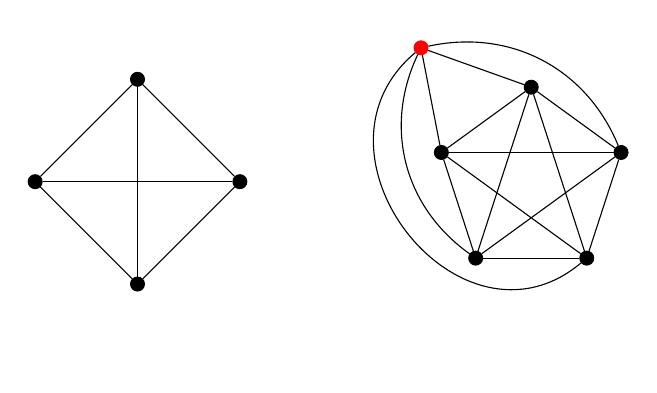
\begin{tikzpicture}[
    mycircle/.style={
        circle,
        draw=black,
        fill=black,
        fill opacity = 1,
        inner sep=0pt,
        minimum size=5pt,
        font=\small},
    nocircle/.style={
        circle,
        draw=black,
        fill=black,
        fill opacity = 1,
        inner sep=0pt,
        minimum size=0.45pt,
        font=\small},
    targetcircle/.style={
        circle,
        draw=red,
        fill=red,
        fill opacity = 1,
        inner sep=0pt,
        minimum size=5pt,
        font=\small},
    myarrow/.style={-},
    dottedarrow/.style={-,dashed},
    thiccarrow/.style={-,line width=0.9pt},
    node distance=1.2cm and 1.5cm
]


\begin{scope}
    \begin{scope}[rotate=90]
        \foreach \x/\y in {0/a,90/b,180/c, 270/d}{ % color in outer layer
        \node[mycircle] (\y) at (canvas polar cs: radius=1.3cm,angle=\x){};
        }
    \end{scope}

    \path[every node/.style={font=\sffamily\small}]
        (a) edge [color=black] (b)
        (a) edge [color=black] (c)
        (a) edge [color=black] (d)
        (b) edge [color=black] (c)
        (b) edge [color=black] (d)
        (c) edge [color=black] (d);
\end{scope}

\begin{scope}[xshift=5cm]
    \begin{scope}[rotate=90]
        \foreach \x/\y in {0/0,72/1,144/2, 216/3, 288/4}{ % color in outer layer
        \node[mycircle] (\y) at (canvas polar cs: radius=1.2cm,angle=\x){};
        }
    \end{scope}

    \path[every node/.style={font=\sffamily\small}]
        (0) edge [color=black] (1)
        (0) edge [color=black] (2)
        (0) edge [color=black] (3)
        (0) edge [color=black] (4)
        (1) edge [color=black] (2)
        (1) edge [color=black] (3)
        (1) edge [color=black] (4)
        (2) edge [color=black] (3)
        (2) edge [color=black] (4)
        (3) edge [color=black] (4);

    \node[targetcircle] (x) at (-1.4, 1.7) {};

    \path[every node/.style={font=\sffamily\small}]
        (x) edge [color=black] (0)
        (x) edge [color=black] (1)
        (x) edge [color=black, bend right=40] (2)
        (x) edge [color=black, out=220, in=-140, looseness=1.5] (3)
        (x) edge [color=black, bend left=40] (4);
\end{scope}
\end{tikzpicture}
\end{document}}
%                 \caption{$t=1$}
%                 \label{2community train series, a}
%             \end{subfigure}
%             \hfill
%             \centering
%             \begin{subfigure}[c]{0.3\textwidth}
%                 \centering
%                 \resizebox{.6\width}{!}{\documentclass{standalone}
\usepackage{amsmath,amssymb,amsthm}
\usepackage{tikz}
\usetikzlibrary{decorations.markings}
\usetikzlibrary{arrows,automata}
\usetikzlibrary{positioning}
\usetikzlibrary{arrows.meta,positioning}

\begin{document}
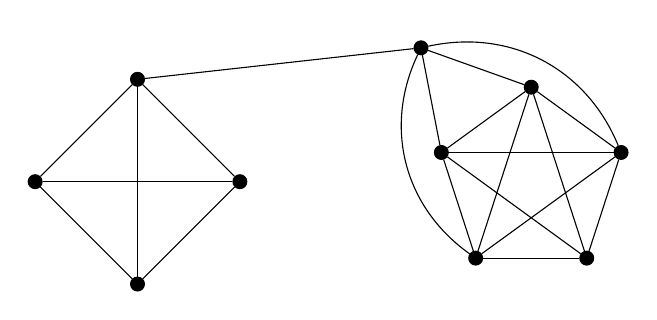
\begin{tikzpicture}[
    mycircle/.style={
        circle,
        draw=black,
        fill=black,
        fill opacity = 1,
        inner sep=0pt,
        minimum size=5pt,
        font=\small},
    nocircle/.style={
        circle,
        draw=black,
        fill=black,
        fill opacity = 1,
        inner sep=0pt,
        minimum size=0.45pt,
        font=\small},
    myarrow/.style={-},
    dottedarrow/.style={-,dashed},
    thiccarrow/.style={-,line width=0.9pt},
    node distance=1.2cm and 1.5cm
]
\begin{scope}
    \begin{scope}[rotate=90]
        \foreach \x/\y in {0/a,90/b,180/c, 270/d}{ % color in outer layer
        \node[mycircle] (\y) at (canvas polar cs: radius=1.3cm,angle=\x){};
        }
    \end{scope}

    \path[every node/.style={font=\sffamily\small}]
        (a) edge [color=black] (b)
        (a) edge [color=black] (c)
        (a) edge [color=black] (d)
        (b) edge [color=black] (c)
        (b) edge [color=black] (d)
        (c) edge [color=black] (d);
\end{scope}

\begin{scope}[xshift=5cm]
    \begin{scope}[rotate=90]
        \foreach \x/\y in {0/0,72/1,144/2, 216/3, 288/4}{ % color in outer layer
        \node[mycircle] (\y) at (canvas polar cs: radius=1.2cm,angle=\x){};
        }
    \end{scope}

    \path[every node/.style={font=\sffamily\small}]
        (0) edge [color=black] (1)
        (0) edge [color=black] (2)
        (0) edge [color=black] (3)
        (0) edge [color=black] (4)
        (1) edge [color=black] (2)
        (1) edge [color=black] (3)
        (1) edge [color=black] (4)
        (2) edge [color=black] (3)
        (2) edge [color=black] (4)
        (3) edge [color=black] (4);

    \node[mycircle] (x) at (-1.4, 1.7) {};

    \path[every node/.style={font=\sffamily\small}]
        (x) edge [color=black] (0)
        (x) edge [color=black] (1)
        (x) edge [color=black, bend right=40] (2)
        (x) edge [color=black, bend left=40] (4)
        (x) edge [color=black] (a);
\end{scope}
\end{tikzpicture}
\end{document}}
%                 \caption{$t=2$}
%                 \label{2community train series, b}
%             \end{subfigure}
%             \hfill
%             \centering
%             \begin{subfigure}[c]{0.3\textwidth}
%                 \centering
%                 \resizebox{.6\width}{!}{\documentclass{standalone}
\usepackage{amsmath,amssymb,amsthm}
\usepackage{tikz}
\usetikzlibrary{decorations.markings}
\usetikzlibrary{arrows,automata}
\usetikzlibrary{positioning}
\usetikzlibrary{arrows.meta,positioning}

\begin{document}
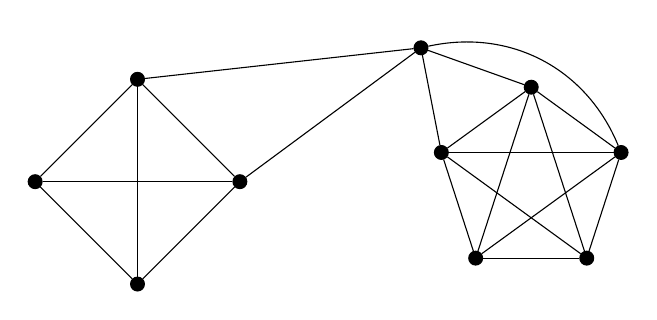
\begin{tikzpicture}[
    mycircle/.style={
        circle,
        draw=black,
        fill=black,
        fill opacity = 1,
        inner sep=0pt,
        minimum size=5pt,
        font=\small},
    nocircle/.style={
        circle,
        draw=black,
        fill=black,
        fill opacity = 1,
        inner sep=0pt,
        minimum size=0.45pt,
        font=\small},
    myarrow/.style={-},
    dottedarrow/.style={-,dashed},
    thiccarrow/.style={-,line width=0.9pt},
    node distance=1.2cm and 1.5cm
]
\begin{scope}
    \begin{scope}[rotate=90]
        \foreach \x/\y in {0/a,90/b,180/c, 270/d}{ % color in outer layer
        \node[mycircle] (\y) at (canvas polar cs: radius=1.3cm,angle=\x){};
        }
    \end{scope}

    \path[every node/.style={font=\sffamily\small}]
        (a) edge [color=black] (b)
        (a) edge [color=black] (c)
        (a) edge [color=black] (d)
        (b) edge [color=black] (c)
        (b) edge [color=black] (d)
        (c) edge [color=black] (d);
\end{scope}

\begin{scope}[xshift=5cm]
    \begin{scope}[rotate=90]
        \foreach \x/\y in {0/0,72/1,144/2, 216/3, 288/4}{ % color in outer layer
        \node[mycircle] (\y) at (canvas polar cs: radius=1.2cm,angle=\x){};
        }
    \end{scope}

    \path[every node/.style={font=\sffamily\small}]
        (0) edge [color=black] (1)
        (0) edge [color=black] (2)
        (0) edge [color=black] (3)
        (0) edge [color=black] (4)
        (1) edge [color=black] (2)
        (1) edge [color=black] (3)
        (1) edge [color=black] (4)
        (2) edge [color=black] (3)
        (2) edge [color=black] (4)
        (3) edge [color=black] (4);

    \node[mycircle] (x) at (-1.4, 1.7) {};

    \path[every node/.style={font=\sffamily\small}]
        (x) edge [color=black] (0)
        (x) edge [color=black] (1)
        (x) edge [color=black, bend left=40] (4)
        (x) edge [color=black] (a)
        (x) edge [color=black] (d);
\end{scope}
\end{tikzpicture}
\end{document}}
%                 \caption{$t=3$}
%                 \label{2community train series, c}
%             \end{subfigure}
%             \caption{First 3 time steps of the simplified, synthetic 2 community network. The red node represents the target node that we are aiming to model. The 4 node and 5 node fully connected components represent the 40 and 50 node communities of the sequence respectively. At each time step, an edge from the target node to the larger community is replaced with and edge from the target node to the smaller community.}
%             \label{2community train series}
%         \end{figure}
%         The 2 community temporal network was selected to test whether this framework can be used to model a node changing communities in systems where there are no other processes occurring. Notably, the movement in the two community system is difficult for the neural network to learn because opposite sets of inputs need to result in the same output. In a simplified version of this system with only the nearest node as input, the input for the model begins as the position of the larger community at roughly $(0,-1)$ \autoref{2community series 1}. This input needs to move the target towards the top left. However, as the sequence progresses, the nearest neighbours will be the small community at roughly $(-1,0)$, which also needs to move the target node towards the top left. 

%     \subsection{Long Tail System}
%         In the long tail network \autoref{longTail train series}, we have a long chain with 50 nodes and a fully connected component with forty nodes at one end of the chain. This is used to orient the embedding and model. The SVD does not take into account the index of the individual node in the adjacency matrix; it only distinguishes based on their distance to each other. Because of this a chain of nodes, even when aligned, could be flipped when it is embedded. That is, between one time step and the next the first node in the chain could be aligned with the last node. With a large, connected group at one end however, that group will always be aligned with itself and so the rest of the chain will also be aligned properly. The target node starts attached to the node that is attached to this large component \autoref{longTail train series, a}. At each time step the target node move one node further down the tail \autoref{longTail train series, b}. Again, this is repeated to generate the training and test data \autoref{longTail train series, c}.
%         \begin{figure}[H]
%             \centering
%             \begin{subfigure}[c]{0.3\textwidth}
%                 \centering
%                 \resizebox{.6\width}{!}{\documentclass{standalone}
\usepackage{amsmath,amssymb,amsthm}
\usepackage{tikz}
\usetikzlibrary{decorations.markings}
\usetikzlibrary{arrows,automata}
\usetikzlibrary{positioning}
\usetikzlibrary{arrows.meta,positioning}

\begin{document}
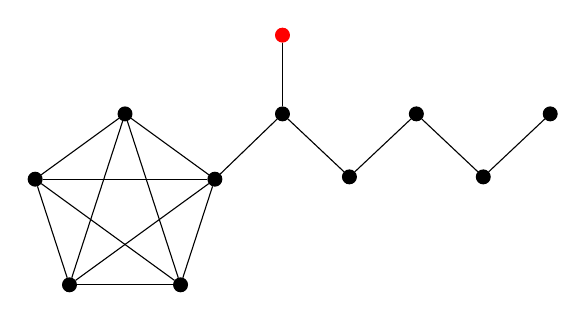
\begin{tikzpicture}[
    mycircle/.style={
        circle,
        draw=black,
        fill=black,
        fill opacity = 1,
        inner sep=0pt,
        minimum size=5pt,
        font=\small},
    nocircle/.style={
        circle,
        draw=black,
        fill=black,
        fill opacity = 1,
        inner sep=0pt,
        minimum size=0.45pt,
        font=\small},
    targetcircle/.style={
        circle,
        draw=red,
        fill=red,
        fill opacity = 1,
        inner sep=0pt,
        minimum size=5pt,
        font=\small},
    myarrow/.style={-},
    dottedarrow/.style={-,dashed},
    thiccarrow/.style={-,line width=0.9pt},
    node distance=1.2cm and 1.5cm
]
\begin{scope}
    \begin{scope}[rotate=90]
        \foreach \x/\y in {0/0,72/1,144/2, 216/3, 288/4}{ % color in outer layer
        \node[mycircle] (\y) at (canvas polar cs: radius=1.2cm,angle=\x){};
        }
    \end{scope}

    \path[every node/.style={font=\sffamily\small}]
        (0) edge [color=black] (1)
        (0) edge [color=black] (2)
        (0) edge [color=black] (3)
        (0) edge [color=black] (4)
        (1) edge [color=black] (2)
        (1) edge [color=black] (3)
        (1) edge [color=black] (4)
        (2) edge [color=black] (3)
        (2) edge [color=black] (4)
        (3) edge [color=black] (4);

    \node[mycircle] (a) at (2, 1.2) {};
    \node[mycircle] (b) at (2.85, 0.4) {};
    \node[mycircle] (c) at (3.7, 1.2) {};
    \node[mycircle] (d) at (4.55, 0.4) {};
    \node[mycircle] (e) at (5.4, 1.2) {};

    \path[every node/.style={font=\sffamily\small}]
        (4) edge [color=black] (a)
        (a) edge [color=black] (b)
        (b) edge [color=black] (c)
        (c) edge [color=black] (d)
        (d) edge [color=black] (e);

    \node[targetcircle] (x) at (2, 2.2) {};

    \path[every node/.style={font=\sffamily\small}]
        (x) edge [color=black] (a);
\end{scope}
\end{tikzpicture}
\end{document}}
%                 \caption{$t=1$}
%                 \label{longTail train series, a}
%             \end{subfigure}
%             \hfill
%             \centering
%             \begin{subfigure}[c]{0.3\textwidth}
%                 \centering
%                 \resizebox{.6\width}{!}{\documentclass{standalone}
\usepackage{amsmath,amssymb,amsthm}
\usepackage{tikz}
\usetikzlibrary{decorations.markings}
\usetikzlibrary{arrows,automata}
\usetikzlibrary{positioning}
\usetikzlibrary{arrows.meta,positioning}

\begin{document}
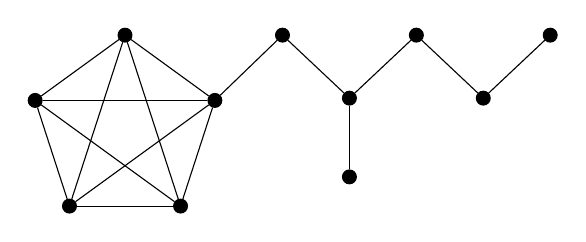
\begin{tikzpicture}[
    mycircle/.style={
        circle,
        draw=black,
        fill=black,
        fill opacity = 1,
        inner sep=0pt,
        minimum size=5pt,
        font=\small},
    nocircle/.style={
        circle,
        draw=black,
        fill=black,
        fill opacity = 1,
        inner sep=0pt,
        minimum size=0.45pt,
        font=\small},
    myarrow/.style={-},
    dottedarrow/.style={-,dashed},
    thiccarrow/.style={-,line width=0.9pt},
    node distance=1.2cm and 1.5cm
]

\begin{scope}
    \begin{scope}[rotate=90]
        \foreach \x/\y in {0/0,72/1,144/2, 216/3, 288/4}{ % color in outer layer
        \node[mycircle] (\y) at (canvas polar cs: radius=1.2cm,angle=\x){};
        }
    \end{scope}

    \path[every node/.style={font=\sffamily\small}]
        (0) edge [color=black] (1)
        (0) edge [color=black] (2)
        (0) edge [color=black] (3)
        (0) edge [color=black] (4)
        (1) edge [color=black] (2)
        (1) edge [color=black] (3)
        (1) edge [color=black] (4)
        (2) edge [color=black] (3)
        (2) edge [color=black] (4)
        (3) edge [color=black] (4);

    \node[mycircle] (a) at (2, 1.2) {};
    \node[mycircle] (b) at (2.85, 0.4) {};
    \node[mycircle] (c) at (3.7, 1.2) {};
    \node[mycircle] (d) at (4.55, 0.4) {};
    \node[mycircle] (e) at (5.4, 1.2) {};

    \path[every node/.style={font=\sffamily\small}]
        (4) edge [color=black] (a)
        (a) edge [color=black] (b)
        (b) edge [color=black] (c)
        (c) edge [color=black] (d)
        (d) edge [color=black] (e);

    \node[mycircle] (x) at (2.85, -0.6) {};

    \path[every node/.style={font=\sffamily\small}]
        (x) edge [color=black] (b);
\end{scope}
\end{tikzpicture}
\end{document}}
%                 \caption{$t=2$}
%                 \label{longTail train series, b}
%             \end{subfigure}
%             \hfill
%             \centering
%             \begin{subfigure}[c]{0.3\textwidth}
%                 \centering
%                 \resizebox{.6\width}{!}{\documentclass{standalone}
\usepackage{amsmath,amssymb,amsthm}
\usepackage{tikz}
\usetikzlibrary{decorations.markings}
\usetikzlibrary{arrows,automata}
\usetikzlibrary{positioning}
\usetikzlibrary{arrows.meta,positioning}

\begin{document}
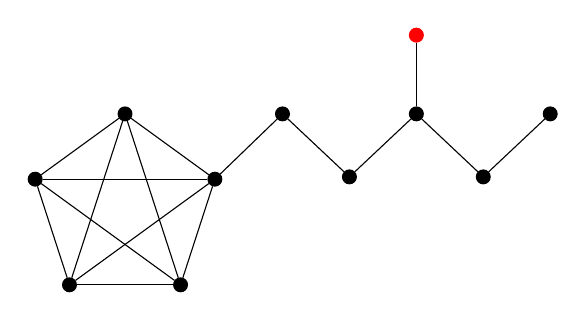
\begin{tikzpicture}[
    mycircle/.style={
        circle,
        draw=black,
        fill=black,
        fill opacity = 1,
        inner sep=0pt,
        minimum size=5pt,
        font=\small},
    nocircle/.style={
        circle,
        draw=black,
        fill=black,
        fill opacity = 1,
        inner sep=0pt,
        minimum size=0.45pt,
        font=\small},
    targetcircle/.style={
        circle,
        draw=red,
        fill=red,
        fill opacity = 1,
        inner sep=0pt,
        minimum size=5pt,
        font=\small},
    myarrow/.style={-},
    dottedarrow/.style={-,dashed},
    thiccarrow/.style={-,line width=0.9pt},
    node distance=1.2cm and 1.5cm
]

\begin{scope}
    \begin{scope}[rotate=90]
        \foreach \x/\y in {0/0,72/1,144/2, 216/3, 288/4}{ % color in outer layer
        \node[mycircle] (\y) at (canvas polar cs: radius=1.2cm,angle=\x){};
        }
    \end{scope}

    \path[every node/.style={font=\sffamily\small}]
        (0) edge [color=black] (1)
        (0) edge [color=black] (2)
        (0) edge [color=black] (3)
        (0) edge [color=black] (4)
        (1) edge [color=black] (2)
        (1) edge [color=black] (3)
        (1) edge [color=black] (4)
        (2) edge [color=black] (3)
        (2) edge [color=black] (4)
        (3) edge [color=black] (4);

    \node[mycircle] (a) at (2, 1.2) {};
    \node[mycircle] (b) at (2.85, 0.4) {};
    \node[mycircle] (c) at (3.7, 1.2) {};
    \node[mycircle] (d) at (4.55, 0.4) {};
    \node[mycircle] (e) at (5.4, 1.2) {};

    \path[every node/.style={font=\sffamily\small}]
        (4) edge [color=black] (a)
        (a) edge [color=black] (b)
        (b) edge [color=black] (c)
        (c) edge [color=black] (d)
        (d) edge [color=black] (e);

    \node[targetcircle] (x) at (3.7, 2.2) {};

    \path[every node/.style={font=\sffamily\small}]
        (x) edge [color=black] (c);
\end{scope}
\end{tikzpicture}
\end{document}}
%                 \caption{$t=3$}
%                 \label{longTail train series, c}
%             \end{subfigure}\\
%             \caption{First 3 time steps of the simplified, synthetic long tail network. The red node represents the target node that we are aiming to model. The fully connected, 5 node component represents a 50 node community at the end of the long tail. At each time step the target node moves one step further along the chain, away from the large community.}
%             \label{longTail train series}
%         \end{figure}    

%         The long tail network was selected because the SVD performs poorly on highly diagonal matrices; that is matrices with long chains.  The long tail problem is difficult for the embedding because a large portion of the network is along the off diagonals; meaning that, to get an accurate embedding, the dimension of the embedding would need to be close to the length of the tail. As such we wish to see how the framework performs when it is presented with a system that the SVD cannot capture.

%     \subsection{Three community System}
%     We also simulate a sequence with three communities. The communities have sizes 40, 35, 30 and have 25, 24, and 23 edges to the target node respectively. In \autoref{3community train series} the communities have been simplified to have sizes of 5, 4, and 3. The target node starts connected to all of these communities with each community having a different number of edges \autoref{3community train series, a}. The community with the fewest edges between the target node will have one edge removed at each time step \autoref{3community train series, b}, and this process is repeated to create the required number of time steps \autoref{3community train series, c}.  
%     \begin{figure}[H]
%         \centering
%         \centering
%         \begin{subfigure}[c]{0.3\textwidth}
%             \centering
%             \resizebox{.6\width}{!}{\documentclass{standalone}
\usepackage{amsmath,amssymb,amsthm}
\usepackage{tikz}
\usetikzlibrary{decorations.markings}
\usetikzlibrary{arrows,automata}
\usetikzlibrary{positioning}
\usetikzlibrary{arrows.meta,positioning}

\begin{document}
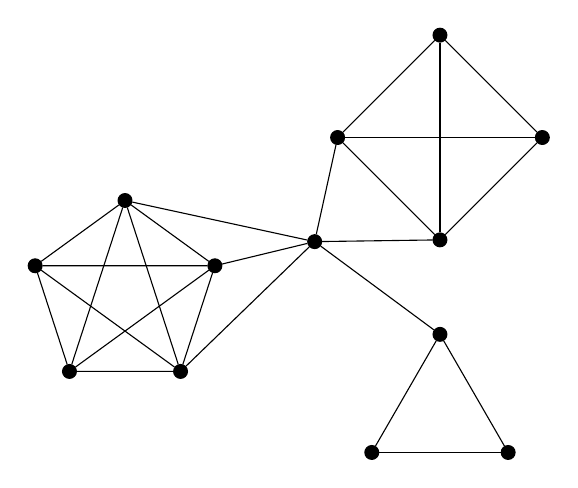
\begin{tikzpicture}[
    mycircle/.style={
        circle,
        draw=black,
        fill=black,
        fill opacity = 1,
        inner sep=0pt,
        minimum size=5pt,
        font=\small},
    nocircle/.style={
        circle,
        draw=black,
        fill=black,
        fill opacity = 1,
        inner sep=0pt,
        minimum size=0.45pt,
        font=\small},
    myarrow/.style={-},
    dottedarrow/.style={-,dashed},
    thiccarrow/.style={-,line width=0.9pt},
    node distance=1.2cm and 1.5cm
]
\begin{scope}
    \begin{scope}[rotate=-90]
        \foreach \x/\y in {0/a,90/b,180/c, 270/d}{ % color in outer layer
        \node[mycircle] (\y) at (canvas polar cs: radius=1.3cm,angle=\x){};
        }
    \end{scope}

    \path[every node/.style={font=\sffamily\small}]
        (a) edge [color=black] (b)
        (a) edge [color=black] (c)
        (a) edge [color=black] (d)
        (b) edge [color=black] (c)
        (b) edge [color=black] (d)
        (c) edge [color=black] (d);
\end{scope}

\begin{scope}[xshift=-4cm, yshift=-2cm, rotate=-72]
    \begin{scope}[rotate=90]
        \foreach \x/\y in {0/0,72/1,144/2, 216/3, 288/4}{ % color in outer layer
        \node[mycircle] (\y) at (canvas polar cs: radius=1.2cm,angle=\x){};
        }
    \end{scope}

    \path[every node/.style={font=\sffamily\small}]
        (0) edge [color=black] (1)
        (0) edge [color=black] (2)
        (0) edge [color=black] (3)
        (0) edge [color=black] (4)
        (1) edge [color=black] (2)
        (1) edge [color=black] (3)
        (1) edge [color=black] (4)
        (2) edge [color=black] (3)
        (2) edge [color=black] (4)
        (3) edge [color=black] (4);

    \node[mycircle] (x) at (0.1, 2.5) {};

    \path[every node/.style={font=\sffamily\small}]
        (x) edge [color=black] (0)
        (x) edge [color=black] (1)
        (x) edge [color=black] (4)
        (x) edge [color=black] (a)
        (x) edge [color=black] (d);
\end{scope}

\begin{scope}[yshift=-3.5cm, xshift=0cm]
    \begin{scope}[rotate=90]
        \foreach \x/\y in {0/0,120/1,240/2}{ % color in outer layer
        \node[mycircle] (\y) at (canvas polar cs: radius=1cm,angle=\x){};
        }
    \end{scope}

    \path[every node/.style={font=\sffamily\small}]
        (0) edge [color=black] (1)
        (0) edge [color=black] (2)
        (1) edge [color=black] (2)
        (x) edge [color=black] (0);
\end{scope}
\end{tikzpicture}
\end{document}}
%             \caption{$t=1$}
%             \label{3community train series, a}
%         \end{subfigure}
%         \hfill
%         \centering
%         \begin{subfigure}[c]{0.3\textwidth}
%             \centering
%             \resizebox{.6\width}{!}{\documentclass{standalone}
\usepackage{amsmath,amssymb,amsthm}
\usepackage{tikz}
\usetikzlibrary{decorations.markings}
\usetikzlibrary{arrows,automata}
\usetikzlibrary{positioning}
\usetikzlibrary{arrows.meta,positioning}

\begin{document}
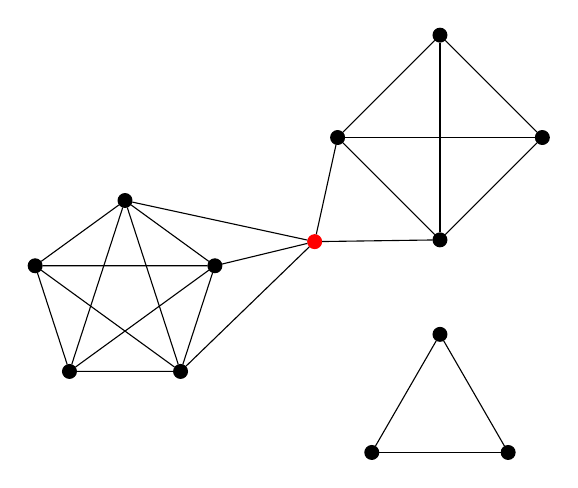
\begin{tikzpicture}[
    mycircle/.style={
        circle,
        draw=black,
        fill=black,
        fill opacity = 1,
        inner sep=0pt,
        minimum size=5pt,
        font=\small},
    nocircle/.style={
        circle,
        draw=black,
        fill=black,
        fill opacity = 1,
        inner sep=0pt,
        minimum size=0.45pt,
        font=\small},
    targetcircle/.style={
        circle,
        draw=red,
        fill=red,
        fill opacity = 1,
        inner sep=0pt,
        minimum size=5pt,
        font=\small},
    myarrow/.style={-},
    dottedarrow/.style={-,dashed},
    thiccarrow/.style={-,line width=0.9pt},
    node distance=1.2cm and 1.5cm
]
\begin{scope}
    \begin{scope}[rotate=-90]
        \foreach \x/\y in {0/a,90/b,180/c, 270/d}{ % color in outer layer
        \node[mycircle] (\y) at (canvas polar cs: radius=1.3cm,angle=\x){};
        }
    \end{scope}

    \path[every node/.style={font=\sffamily\small}]
        (a) edge [color=black] (b)
        (a) edge [color=black] (c)
        (a) edge [color=black] (d)
        (b) edge [color=black] (c)
        (b) edge [color=black] (d)
        (c) edge [color=black] (d);
\end{scope}

\begin{scope}[xshift=-4cm, yshift=-2cm, rotate=-72]
    \begin{scope}[rotate=90]
        \foreach \x/\y in {0/0,72/1,144/2, 216/3, 288/4}{ % color in outer layer
        \node[mycircle] (\y) at (canvas polar cs: radius=1.2cm,angle=\x){};
        }
    \end{scope}

    \path[every node/.style={font=\sffamily\small}]
        (0) edge [color=black] (1)
        (0) edge [color=black] (2)
        (0) edge [color=black] (3)
        (0) edge [color=black] (4)
        (1) edge [color=black] (2)
        (1) edge [color=black] (3)
        (1) edge [color=black] (4)
        (2) edge [color=black] (3)
        (2) edge [color=black] (4)
        (3) edge [color=black] (4);

    \node[targetcircle] (x) at (0.1, 2.5) {};

    \path[every node/.style={font=\sffamily\small}]
        (x) edge [color=black] (0)
        (x) edge [color=black] (1)
        (x) edge [color=black] (4)
        (x) edge [color=black] (a)
        (x) edge [color=black] (d);
\end{scope}

\begin{scope}[yshift=-3.5cm, xshift=0cm]
    \begin{scope}[rotate=90]
        \foreach \x/\y in {0/0,120/1,240/2}{ % color in outer layer
        \node[mycircle] (\y) at (canvas polar cs: radius=1cm,angle=\x){};
        }
    \end{scope}

    \path[every node/.style={font=\sffamily\small}]
        (0) edge [color=black] (1)
        (0) edge [color=black] (2)
        (1) edge [color=black] (2);
\end{scope}
\end{tikzpicture}
\end{document}}
%             \caption{$t=2$}
%             \label{3community train series, b}            
%         \end{subfigure}
%         \hfill
%         \centering
%         \begin{subfigure}[c]{0.3\textwidth}
%             \centering
%             \resizebox{.6\width}{!}{\documentclass{standalone}
\usepackage{amsmath,amssymb,amsthm}
\usepackage{tikz}
\usetikzlibrary{decorations.markings}
\usetikzlibrary{arrows,automata}
\usetikzlibrary{positioning}
\usetikzlibrary{arrows.meta,positioning}

\begin{document}
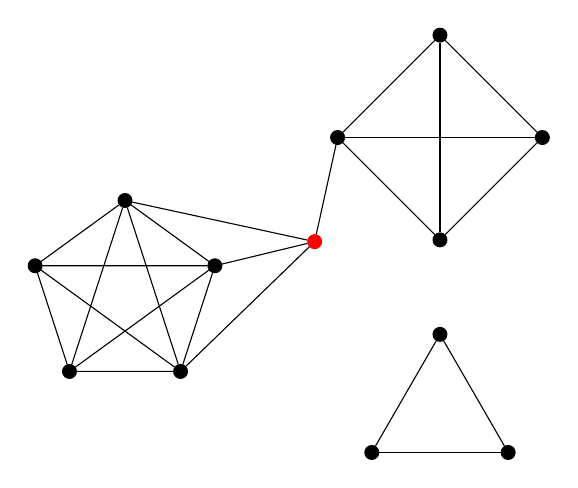
\begin{tikzpicture}[
    mycircle/.style={
        circle,
        draw=black,
        fill=black,
        fill opacity = 1,
        inner sep=0pt,
        minimum size=5pt,
        font=\small},
    nocircle/.style={
        circle,
        draw=black,
        fill=black,
        fill opacity = 1,
        inner sep=0pt,
        minimum size=0.45pt,
        font=\small},
    targetcircle/.style={
        circle,
        draw=red,
        fill=red,
        fill opacity = 1,
        inner sep=0pt,
        minimum size=5pt,
        font=\small},
    myarrow/.style={-},
    dottedarrow/.style={-,dashed},
    thiccarrow/.style={-,line width=0.9pt},
    node distance=1.2cm and 1.5cm
]
\begin{scope}
    \begin{scope}[rotate=-90]
        \foreach \x/\y in {0/a,90/b,180/c, 270/d}{ % color in outer layer
        \node[mycircle] (\y) at (canvas polar cs: radius=1.3cm,angle=\x){};
        }
    \end{scope}

    \path[every node/.style={font=\sffamily\small}]
        (a) edge [color=black] (b)
        (a) edge [color=black] (c)
        (a) edge [color=black] (d)
        (b) edge [color=black] (c)
        (b) edge [color=black] (d)
        (c) edge [color=black] (d);
\end{scope}

\begin{scope}[xshift=-4cm, yshift=-2cm, rotate=-72]
    \begin{scope}[rotate=90]
        \foreach \x/\y in {0/0,72/1,144/2, 216/3, 288/4}{ % color in outer layer
        \node[mycircle] (\y) at (canvas polar cs: radius=1.2cm,angle=\x){};
        }
    \end{scope}

    \path[every node/.style={font=\sffamily\small}]
        (0) edge [color=black] (1)
        (0) edge [color=black] (2)
        (0) edge [color=black] (3)
        (0) edge [color=black] (4)
        (1) edge [color=black] (2)
        (1) edge [color=black] (3)
        (1) edge [color=black] (4)
        (2) edge [color=black] (3)
        (2) edge [color=black] (4)
        (3) edge [color=black] (4);

    \node[targetcircle] (x) at (0.1, 2.5) {};

    \path[every node/.style={font=\sffamily\small}]
        (x) edge [color=black] (0)
        (x) edge [color=black] (1)
        (x) edge [color=black] (4)
        (x) edge [color=black] (d);
\end{scope}

\begin{scope}[yshift=-3.5cm, xshift=0cm]
    \begin{scope}[rotate=90]
        \foreach \x/\y in {0/0,120/1,240/2}{ % color in outer layer
        \node[mycircle] (\y) at (canvas polar cs: radius=1cm,angle=\x){};
        }
    \end{scope}

    \path[every node/.style={font=\sffamily\small}]
        (0) edge [color=black] (1)
        (0) edge [color=black] (2)
        (1) edge [color=black] (2);
\end{scope}
\end{tikzpicture}
\end{document}}
%             \caption{$t=3$}
%             \label{3community train series, c}
%         \end{subfigure}
%         \caption{First 3 time steps of the simplified, synthetic 3 community networks. The red node represents the target node which we aim to model. The 3, 4, and 5 node components represent the 30, 35, and 40 node communities respectively. At each time step the one edge is removed between the target node and the community it has the fewest connections with.}
%         \label{3community train series}
%     \end{figure}
     
%     The three community was chosen as a best case scenario system to model. It has been constructed to avoid the challenges that are posed by the 2 community and long tail systems. That is, because in this system the target node is moving away from its least similar community, not moving from one community to another, it is not required to overcome the issue of symmetrical input. And because there are no long tails in this system, the SVD is able to capture a lot of the system with a low dimensional.

% \end{section}

\begin{section}{Results and Discussion}
    \subsection{Network Prediction}
    To compare our models, we look at the loss of the predictions. This includes the loss from the SVD.
    
    To find the approximation of the edges of node $i$, $_tA_{i,\cdot}$. We use: 
    \begin{align}
        _tA_{i,\cdot} &\approxeq (\bar p) _t\hat A
    \end{align}
    Where $\bar p$ is the location of the node $i$ in the embedding at time $t$.

    To find calculate the loss of our prediction at time $t$, we use:
    \begin{align}
        L = ||_tA_{i,\cdot} - (\bar p) _t\hat A||_1
    \end{align}
    
    When we do this for the SVD, NN, and symbolic regression, we get \autoref{loss_table}.
    \begin{figure}
        \begin{center}
            \begin{tabular}{| m{0.17\textwidth} | m{0.25\textwidth} | m{0.25\textwidth} | m{0.25\textwidth} |}
                \hline
                Sequence & Embedding Loss & Neural Network Prediction Loss & Symbolic Regression Prediction Loss\\ 
                \hline
                \hline
                2 Community & 41.67 & 47.91 & 35.11\\ 
                \hline 
                Long Tail & 2.408 & 1.193 & 2.524 \\ 
                \hline 
                3 Community & 35.43 & 35.50 & 35.57 \\ 
                \hline 
            \end{tabular}
            \end{center}
            \caption{A summary of the mean loss of each prediction at the fifth time step. The embedding loss comes from the true target node and loss is only introduced by the SVD. The neural network and symbolic prediction loss comes from the RDPG being reconstructed but with the position of the target node replaced with the location of the respective prediction. Loss is calculated as the total number of incorrectly predicted edges. That is an edge not being present when it should as well as the reverse.}
            \label{loss_table}
    \end{figure}

    The loss of one system should not be compared with another. That is the 2 community losses should not be compared to the long tail. This is because the long tail system will only ever have one edge to predict, whereas the 2 community will have 50 edges that need to be predicted.

    Instead, we may compare predictions within the same system. However, we do not see much difference between these predictions, and so we plot our predictions at each time step to further understand the behavior of our framework.

    For each of these systems, we took embedded the temporal network in two dimensions at each time step. The temporal embeddings were then divided into a training set of 20 and a testing set of 15. The output of the trained neural networks was then used to train a symbolic regression model that could use a simple set of addition, subtraction, division, and multiplication. \\
    In fig \autoref{2community series}, \autoref{longtail series},\autoref{3community series} the green points are the embedded coordinates of the node in each of the communities. Each cluster is one separate community. The orange point is the true coordinate of the embedded target node at each time step. The blue point is our model prediction from the true target node at the first time step. As the time progresses, we see the true node move from one community cluster to the other. This is expected from the embedding; the target node starts as very similar to the first community (as it has many connections with nodes in that community) and as time progresses, it gradually becomes less and less similar to the first community and more similar to the second (as the edges between the target node and the first community are replaced with edges to the second community). As such, we see the target node move towards the second community.

    \begin{subsection}{2 Community}
        \begin{figure}
            \foreach \i in {1,...,15} {%
                \begin{subfigure}[p]{0.3\textwidth}
                    \includegraphics[width=\linewidth]{../Code/Plots/Test Only/2communities/2communities \i \space small net.png}
                    \caption{t=\i}
                    \label{2community series \i}
                \end{subfigure}\quad
            }
            \caption{2 Community test series. This series shows the comparison of the neural network model, the symbolic regression model trained on the neural network model, and the true solution of the two community system.}
            \label{2community series}
        \end{figure}
        We see the neural network model quickly jumps to around $(-0.5,-0.5)$ where it sits for the entire simulation. This happened across many training periods; either a few time steps after the training period or right at the end of it, the neural network model moved towards a stable point where it remained for the test period.

        In contrast, the symbolic regression predicted the location of the target node very well at the beginning of the test period, but after about 5 steps starts to drift away. 
        
        The poor predictive behaviour of the neural network especially may be attributed to this being a symmetrical problem. That is the same set of distances as input into the neural network, the target node needs to move away from its nearest neighbours in the first half, then move towards its nearest neighbours in the second half. Potential ways of breaking this symmetry may be to include information of the previous time step, or to include the absolute position of the target node as input into the neural network.

        Notably, using the small neural network model to train the symbolic regression gave much better predictions than the large neural network\ref{2community series large neural network}. 
        
        % It is interesting to see the symbolic regression model perform so much more poorly than the neural network model in this system. When we view the training section of the data, we see that there is a downward curve in the neural network predictions towards the end of the training data. It seems that the symbolic regression model picked this up and continued the downward trajectory throughout the test data. This downward curve may be because the problem that we are trying to solve is symmetrical. That is 
    \end{subsection}

    \begin{subsection}{Long Tail}
        \begin{figure} 
            \foreach \i in {1,...,15} {%
                \begin{subfigure}[p]{0.3\textwidth}
                    \includegraphics[width=\linewidth]{../Code/Plots/Test Only/longTail/longTail \i \space small net.png}
                    \caption{t=\i}
                    \label{longtail series \i}
                \end{subfigure}\quad
            }
            \caption{Long Tail test series. This series shows the comparison of the neural network model, the symbolic regression model trained on the neural network model, and the true solution of the long tail system.}
            \label{longtail series}
        \end{figure}
        In fig \autoref{longtail series} we see the true embedding of the target node jump from one arm to the other at each time step. It is clear that neither the symbolic regression model nor the neural network model capture this movement. We also see that the symbolic regression model maintains a relatively stable position when compared to the neural network model.

        We see that neither the neural network model capture the movement of the target node to any real extent. One reason for this may again be an issue of symmetrical input. The distances from the k nearest neighbours to the target node do not seem to change much as the target node jumps from one arm to the other, but the neural network somehow needs to learn to jump left then right at alternating time steps. The solutions to this would be the same as for the two community system.
    \end{subsection}

    \begin{subsection}{Three Community}
        \begin{figure}
            \foreach \i in {1,...,15} {%
                \begin{subfigure}[p]{0.3\textwidth}
                    \includegraphics[width=\linewidth]{../Code/Plots/Test Only/3community/3community \i \space small net.png}
                    \caption{t=\i}
                    \label{3community series \i}
                \end{subfigure}\quad
            }
            \caption{3 community test series. This series shows the comparison of the neural network model, the symbolic regression model trained on the neural network model, and the true solution of the 3 community system.}
            \label{3community series}
        \end{figure}
        In fig \autoref{3community series} we again, as the edges between the community with the fewest edges are removed, we see the target node move away from it in the embedding and towards the other two clusters of points (communities).

        For the first ten time steps, we see similar behaviour between the neural network model and the neural network model. However, around the eleventh time step, the symbolic regression model begins to diverge from the neural network. The symbolic regression moves back towards the target node towards the end. This could indicate that the symbolic regression is a somewhat more robust model when extrapolating, but more testing should be done to corroborate this.

        Notably the symbolic regression trained on the large neural network performed extremely well, while the predictions of the large neural network model itself did not seem to make any significant improvement\ref{3community series large neural network}. This may indicate that...XXXXX  
        % In the neural network only model, we see the prediction follow the true target node very closely at first. We then see the node drift further and further from the true target node. In contrast, the symbolic regression model remains much closer to the true position of the target node as the test data progresses. We see the symbolic regression move slightly ahead of the true location at first, but this distance remains relatively constant thereafter.

        In the neural network model, we see the prediction remain at close to its initial location for the duration of the test. This seems to indicate an attractor in the model.

        In contrast, we see that the symbolic regression model quickly moves ahead of the true location where it remains for the duration of the test.

        % This was by far the largest improvement between the neural network and the symbolic regression. This could be because this system had the least difference between the training predictions and the true position of the target node. At the end of the test data we see the true target node move towards the origin. This is because it now only has edges to one community and so at each timestep it removes one of these. If this had continued, the target node would have no edges. Nodes with no edges are mapped to the origin. When this happened, the symbolic regression model prediction began to move further from the true node.

        
        \subsection{Summary}
        We see a large difference in the training predictions between the 2 and 3 community systems. In the 2 community system, even in the training period, the predictions tended to wander and be less accurate. Whereas the 3 community training predictions remained very close to the true target node. The movement of the target node in the embedding was very similar between the two systems, and so the difference seems to be that the 2 community has symmetrical inputs.

        These were trained on a relatively small neural network (one hidden layer of 64 nodes), when training this small network one of the issues we encountered was that the weights would become stuck in local minima. To manage this we found that simulate annealing was helpful. When training on a larger network (4 hidden layers (64,8,8,8)) this does not seem to be as much of a problem.
    \end{subsection}

\end{section}

\begin{section}{Conclusion}
    In this paper, we proposed a novel framework for modelling temporal networks. We then tested this framework on three types of small, synthetic network sequences. Throughout these tests the neural network performed generally more poorly than the symbolic regression model, with the large three community sequence being especially notable due to th symbolic regression remaining so close to the target node throughout the test period. 
\end{section} 


\printbibliography

\end{document} 

% draft for miguel
% all absolute pos of nodes
% polar positions

% questions for Giulio:
%     Why both NN and sym reg not just sym reg
%     Why cos dist 